\documentclass{article}
\usepackage[utf8]{inputenc}
\usepackage[includeheadfoot, margin=1em,headheight=2em]{geometry}
\usepackage{titling}
\geometry{a4paper, left=2cm, right=2cm, top=2cm, bottom=2cm}
\usepackage{graphicx}
\providecommand{\versionnumber}{1.0.0}
\usepackage{enumitem}
\usepackage{array}
\usepackage[italian]{babel}
\newcolumntype{P}[1]{>{\centering\arraybackslash}p{#1}}
\renewcommand{\arraystretch}{1.5} % Default value: 1
\setlength{\droptitle}{-6em}
\usepackage{amsmath}
\usepackage{amsfonts}

%font
\usepackage[defaultfam,tabular,lining]{montserrat}
\usepackage[T1]{fontenc}
\renewcommand*\oldstylenums[1]{{\fontfamily{Montserrat-TOsF}\selectfont #1}}

%custom bold 
\usepackage[outline]{contour}
\usepackage{xcolor}
\newcommand{\custombold}{\contour{black}}

%table colors
\usepackage{color, colortbl}
\definecolor{Blue}{rgb}{0.51,0.68,0.79}
\definecolor{LightBlue}{rgb}{0.82,0.87,0.90}
\definecolor{LighterBlue}{rgb}{0.93,0.95,0.96}

%Header
\usepackage{fancyhdr, xcolor}
\pagestyle{fancy}
\let\oldheadrule\headrule% Copy \headrule into \oldheadrule
\renewcommand{\headrule}{\color{Blue}\oldheadrule}% Add colour to \headrule
\renewcommand{\headrulewidth}{0.2em}
\fancyhead[L]{Studio Grafi}
\fancyhead[C]{Samuele Vignotto}
\fancyhead[R]{
\includegraphics[height=1cm]{Logo/Y_LOGO-SOLO.png}}
\setcounter{secnumdepth}{0}

\title{\Huge{\textbf{Grafi}}\vspace{-1em}}
\author{Samuele Vignotto}
\date{}
\begin{document}
\maketitle
\begin{figure}[h]
  \centering
  
\includegraphics[width=6cm, height=6cm]{Logo/Y_LOGO-SOLO.png}
  \label{fig:immagine}
\end{figure}

\newpage
\tableofcontents
\newpage

\section{Introduzione}
I grafi sono una struttura dati e un linguaggio universale per descrivere sistemi complessi. Essi consistono di nodi e archi che rappresentano le relazioni tra entità. La teoria dei grafi fornisce una base matematica per analizzare, comprendere e apprendere dai sistemi del mondo reale.

\section{Concetti fondamentali dei grafi}

Un grafo \(G = (V, E)\) è una struttura matematica composta da un insieme di vertici \(V\) e un insieme di archi \(E\) che collegano coppie di vertici. Questa definizione generale dei grafi permette di modellare una vasta gamma di situazioni e problemi reali, dalle reti di comunicazione ai sistemi biologici, dalle interazioni sociali ai percorsi logistici. I grafi si possono distinguere in non orientati e orientati, pesati e non pesati, e nel caso in cui contengano vari tipi di archi e nodi, sono noti come grafi eterogenei.\\
Nei grafi non orientati, gli archi non hanno una direzione specifica, il che significa che la connessione tra due vertici è bidirezionale. Questo tipo di grafo è particolarmente utile per rappresentare relazioni simmetriche, come le amicizie in una rete sociale o le strade bidirezionali in una mappa. Al contrario, nei grafi orientati, ogni arco ha una direzione, indicando un percorso unidirezionale tra due vertici. Questa rappresentazione è fondamentale in situazioni dove la direzione della relazione è significativa, come nel caso delle transazioni finanziarie o delle dipendenze tra task in un progetto.\\
I grafi pesati si caratterizzano per avere archi ai quali sono associati dei pesi. Questi pesi possono rappresentare varie misure, come la distanza tra due località in una rete stradale, il costo di una transazione, o la capacità di una connessione di rete. La possibilità di associare pesi agli archi amplia notevolmente le applicazioni dei grafi, permettendo di modellare scenari complessi in modo più accurato. I grafi eterogenei, invece, presentano nodi e archi di diversi tipi e attributi. Questa eterogeneità permette di rappresentare sistemi dove le unità fondamentali non sono omogenee, come nei network biologici dove differenti tipi di proteine interagiscono tra loro, o nei social network dove esistono diverse forme di interazioni tra utenti.\\
La rappresentazione dei grafi è comunemente effettuata tramite matrici di adiacenza o liste di adiacenza. La matrice di adiacenza \(A\) per un grafo con \(n\) nodi è una matrice \(n \times n\) in cui l'elemento \(A[i][j]\) indica la presenza o il peso di un arco tra i nodi \(i\) e \(j\). Questa rappresentazione è particolarmente utile per grafi densi, dove la maggior parte delle coppie di nodi sono connesse. In alternativa, le liste di adiacenza elencano per ciascun nodo tutti i nodi a esso collegati, offrendo una rappresentazione più efficiente in termini di spazio per grafi sparsi, dove le connessioni tra i nodi sono relativamente poche rispetto al numero totale di possibili connessioni.\\
I grafi trovano applicazione in numerosi algoritmi, tra cui la ricerca in ampiezza e la ricerca in profondità, che sono fondamentali per l'esplorazione dei grafi stessi. Questi algoritmi permettono di visitare tutti i nodi di un grafo in modo sistematico, trovando percorsi, verificando la connettività e individuando componenti connesse. L'algoritmo di Dijkstra, utilizzato per trovare i percorsi minimi, è essenziale in molte applicazioni pratiche, come la navigazione GPS, dove è necessario trovare il percorso più breve tra due punti. PageRank, un altro algoritmo basato sui grafi, è impiegato nei motori di ricerca per valutare l'importanza delle pagine web, sfruttando la struttura dei link tra le pagine per determinare la rilevanza di ciascuna.

\subsection{Rappresentazioni e statistiche dei grafi}

Una modalità comune di rappresentare i grafi è attraverso le matrici di adiacenza, dove la presenza di un arco tra due nodi è indicata da un valore positivo nella cella corrispondente della matrice. Questa rappresentazione è semplice e permette di effettuare operazioni matematiche e algebriche sui grafi utilizzando strumenti di algebra lineare. Tuttavia, per grafi molto grandi e sparsi, le matrici di adiacenza possono risultare inefficienti in termini di memoria, rendendo preferibile l'uso delle liste di adiacenza. Le liste di adiacenza elencano per ogni nodo tutti i nodi a esso collegati, risultando particolarmente utili per grafi con un numero relativamente basso di archi rispetto ai nodi.\\
Le statistiche dei grafi offrono informazioni preziose sulle caratteristiche strutturali del grafo. Il grado dei nodi, per esempio, indica il numero di connessioni che ciascun nodo ha con altri nodi. Questa misura è fondamentale per comprendere la distribuzione delle connessioni all'interno del grafo e per identificare nodi altamente connessi, che possono svolgere ruoli cruciali nella rete. Altre misure di centralità, come la centralità di autovettore, forniscono una misura più sofisticata dell'importanza di un nodo, considerando non solo i collegamenti diretti, ma anche quelli indiretti attraverso altri nodi. La centralità di autovettore è particolarmente utile per identificare nodi che sono influenti non solo per le loro connessioni immediate, ma anche per la loro posizione strategica nella rete.\\
Il coefficiente di clustering, invece, misura la tendenza dei nodi a formare cluster o gruppi densi. Questo coefficiente indica la densità locale di collegamenti nel grafo, fornendo informazioni sulla struttura comunitaria della rete. Un alto coefficiente di clustering suggerisce che i nodi tendono a formare comunità strette, dove i vicini di un nodo sono spesso connessi tra loro, mentre un basso coefficiente indica una struttura più dispersa e meno comunitaria. Questi concetti sono essenziali per comprendere la struttura e le dinamiche dei grafi, con applicazioni che spaziano dalla sociologia, dove si studiano le interazioni sociali, alla biologia, dove si analizzano le reti di interazioni tra proteine, dall'informatica, dove si progettano algoritmi efficienti per il web, alla fisica dei sistemi complessi, dove si modellano fenomeni emergenti in reti di grande scala.

\subsection{Concetti di centralità e coefficiente di clustering}

Il grado di un nodo è una misura fondamentale che indica il numero di collegamenti di un nodo con altri nodi. Questa semplice metrica è uno dei primi passi per analizzare un grafo, fornendo una panoramica sulla connettività dei singoli nodi. Un nodo con un alto grado è considerato un nodo hub, il che significa che ha molte connessioni con altri nodi e potrebbe giocare un ruolo cruciale nella trasmissione di informazioni o nella stabilità della rete.\\
La centralità, e in particolare la centralità di autovettore, offre una misura più complessa dell'importanza di un nodo all'interno del grafo. Questo concetto considera non solo il numero di collegamenti diretti di un nodo, ma anche la qualità e quantità dei collegamenti indiretti attraverso altri nodi. La centralità di autovettore è utile in molti contesti pratici, come nell'analisi delle reti sociali per identificare individui influenti o nelle reti di comunicazione per individuare nodi critici che facilitano il flusso di informazioni.\\
Il coefficiente di clustering misura la tendenza dei nodi a formare cluster o gruppi densi. Questo coefficiente è calcolato come il rapporto tra il numero effettivo di archi tra i vicini di un nodo e il numero massimo possibile di tali archi. Un alto coefficiente di clustering indica che i nodi tendono a formare gruppi locali densi, suggerendo una struttura comunitaria forte all'interno del grafo. Questa proprietà è spesso osservata in reti sociali, dove le persone tendono a formare gruppi di amici stretti, ma è rilevante anche in molti altri tipi di reti, come quelle biologiche e tecnologiche.\\
Questi concetti sono essenziali per comprendere la struttura e le dinamiche dei grafi. Analizzando il grado, la centralità e il coefficiente di clustering, è possibile ottenere una visione dettagliata delle proprietà del grafo e delle interazioni tra i suoi nodi. Queste analisi sono fondamentali per sviluppare algoritmi efficienti e per applicazioni pratiche in numerosi campi, dalla sociologia alla biologia, dall'informatica alla fisica dei sistemi complessi.

\section{Grafi nel Process Mining}

Il process mining utilizza rappresentazioni basate su grafi per modellare e analizzare i processi aziendali. Attraverso l'analisi dei log di eventi, che sono registrazioni cronologiche delle attività svolte all'interno di un'azienda, i dati vengono trasformati in grafi diretti. In questi grafi, i nodi rappresentano le attività eseguite e gli archi rappresentano l'ordine di esecuzione delle attività stesse. Questa rappresentazione grafica dei processi aiuta non solo a scoprire come vengono realmente svolti i processi aziendali, ma anche a monitorarli in tempo reale e a individuare aree di miglioramento.

\subsection{Log di eventi e modelli di processo}

I log di eventi costituiscono una fonte di dati fondamentale nel process mining. Essi registrano in modo dettagliato le varie attività che compongono i processi aziendali, indicando per ciascuna attività l'istante temporale in cui è stata eseguita. Questi log possono essere elaborati e trasformati in modelli di processo che vengono rappresentati come grafi. In tali modelli, i nodi corrispondono alle attività eseguite e gli archi rappresentano la sequenza temporale con cui queste attività vengono svolte. Questo tipo di rappresentazione permette un'analisi dettagliata dei processi aziendali, consentendo di identificare inefficienze, colli di bottiglia e altre problematiche operative. Analizzando i modelli di processo è possibile ottimizzare le attività, ridurre i tempi di esecuzione e migliorare la produttività complessiva.

\subsection{Reti di Petri}

Uno degli strumenti più potenti e utilizzati nel campo del process mining è la rete di Petri. Le reti di Petri offrono una rappresentazione grafica dei flussi di lavoro, che consente di modellare e analizzare processi complessi. Ogni rete di Petri è composta da posti, transizioni e archi che collegano questi elementi. I posti rappresentano stati o condizioni, mentre le transizioni rappresentano eventi o attività che modificano tali stati. Gli archi indicano le relazioni di causalità tra stati e attività. Questa struttura permette di identificare facilmente colli di bottiglia, deviazioni dal processo previsto e aree in cui è possibile ottimizzare i flussi di lavoro. Le reti di Petri sono particolarmente efficaci nella rappresentazione di processi paralleli e sincroni, dove più attività possono essere svolte contemporaneamente o richiedono una coordinazione precisa.

\subsubsection{Come funziona la rete di Petri}

Una rete di Petri del tipo posto/transizione (o rete P/T) è una struttura composta da due insiemi e due matrici.
\[
N = \{ P,T,Pre, Post \}
\]

La rappresentazione grafica è un grafo orientato (digrafo) con archi pesati formato da posti e transizioni.

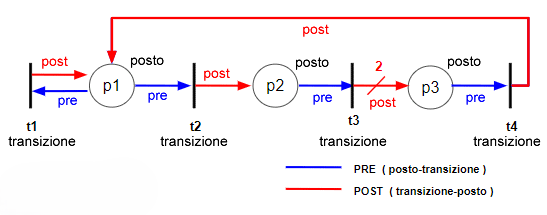
\includegraphics{imgGrafi/rete-di-petri-spiegazione.png}\\

I posti ($p$) sono sono rappresentati da cerchi. Formalmente l'insieme dei posti è indicato con la lettera $P$.
\[
P = \{ p_1, p_2, p_3, ... \}
\]

Le transizioni ($t$) sono rappresentate da barre o da rettangoli. Formalmente, l'insieme delle transizioni è indicato con la lettera $T$.
\[
T = \{ t_1, t_2, t_3, ... \}
\]
Sia i posti che le transizioni sono nodi del digrafo. Sono indicati con un simbolo diverso per distinguerli tra loro. Si presume che $P$ e $T$ siano insiemi disgiunti ossia $P \cap T = \emptyset$ \\

Gli archi dai posti alle transizioni sono detti archi pre-incidenza e sono rappresentati da una matrice $Pre(p,t)$. \\
Si chiama "Pre" perché conta gli archi in entrata (input) delle transizioni.
\begin{center}
    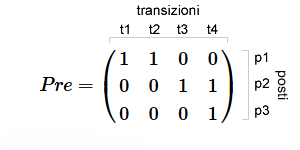
\includegraphics{imgGrafi/matrice-pre-incidenza-esempio.png}
\end{center}

Gli archi dalle transizioni ai posti sono detti archi post-incidenza e sono rappresentati da una matrice $Post(p,t)$. \\
Si chiama "Post" perché conta gli archi in uscita (output) delle transizioni.
\begin{center}
    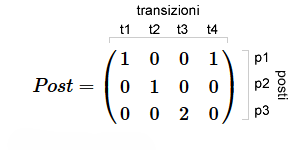
\includegraphics{imgGrafi/matrice-post-incidenza-esempio.png}
\end{center}
In entrambi i casi i posti sono disposti in riga mentre le transizioni sono disposte in colonna. Gli elementi della matrice sono interi non negativi che indicano la presenza dell'arco (1) o l'assenza (0). Se l'intero è un numero maggiore di 1, il numero indica la quantità di archi.\\

Spesso le due matrici Pre e Post sono unite in un'unica matrice in forma compatta, detta matrice di incidenza.

\[
C=Post-Pre = \begin{pmatrix} 1-1 & 0-1 & 0 & 1 \\ 0 & 1 & 0-1 & 0-1 \\ 0 & 0 & 2 & 0-1 \end{pmatrix} = \begin{pmatrix} 0 & -1 & 0 & 1 \\ 0 & 1 & -1 & -1 \\ 0 & 0 & 2 & -1 \end{pmatrix}
\]

Ogni elemento della matrice di incidenza è la somma algebrica dei rispettivi elementi nelle matrici Post e Pre.

\[
C(p,t)=Post(p,t)-Pre(p,t)
\]
La forma comporta una perdita di informazioni. Ad esempio, se un posto e una transizione hanno un eguale numero di archi reciproci tra loro (cappio) nella matrice di incidenza la differenza è comunque pari a zero, come se non ci fosse nulla. In pratica, la rete appare sempre senza cappi (rete pura) anche se ci sono.\\
A ogni elemento è associato un insieme con gli elementi associati in entrata e in uscita.\\
Generalmente si mette il simbolo star prima dell'elemento (*n) per indicare i collegamenti in entrata, dopo il nome (n*) per quelli in uscita.\\
Per esmpio: il posto
\[p_1\]
ha i seguenti collegamenti in entrata
\[*p_1={t_1,t_4}\]
e in uscita
\[p_1*={t_1,t_2}\]
Lo stesso si può fare per le transizioni. La transizione t1 ha i seguenti collegamenti in entrata
\[*t_1={p_1}\]
e in uscita
\[t_1*={p_1}\]

\subsubsection{Esempio pratico}

Ho una rete composta da tre posti
\[
P = \{ p_1, p_2, p_3 \}
\]

e da quattro transizioni
\[
T = \{ t_1, t_2, t_3, t_4 \}
\]

La matrice pre-incidenza (posti-transizioni) conta gli archi in entrata nelle transizioni ed è la seguente
\[
Pre = \begin{pmatrix} 1 & 1 & 0 & 0 \\ 0 & 0 & 1 & 0 \\ 0 & 0 & 0 & 1 \end{pmatrix}
\]

La matrice post-incidenza (transizioni-posti) conta gli archi in uscita dalla transizioni ed è la seguente
\[
Post = \begin{pmatrix} 1 & 0 & 0 & 1 \\ 0 & 1 & 0 & 0 \\ 0 & 0 & 2 & 0 \end{pmatrix}
\]

Per rappresentare il digrafo disegno un cerchio per ogni posto P e una barra (o rettangolo) pr ogni transizione T.\\
\begin{center}
    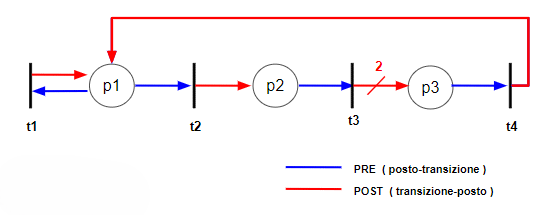
\includegraphics{imgGrafi/esempio-rete-di-petri.png}
\end{center}
Poi li collego tra loro con degli archi orientati secondo le indicazioni delle matrici pre e post incidenza:
\begin{itemize}
    \item Per ogni intero positivo della matrice di pre-incidenza aggiungo nel digrafo un arco di colore rosso dal posto alla transizione.
    \item Per ogni intero positivo della matrice di post-incidenza aggiungo nel digrafo un arco di colore blu dalla transizione al posto.
\end{itemize}
Gli elementi uguali a zero nella matrice indicano l'assenza dell'arco. Quindi, li ignoro. Viceversa la presenza di un intero positivo indica la presenza dell'arco. Se l'intero n è maggiore di 1, vuol dire che ci sono n archi da disegnare. In questo caso è preferibile scrivere un solo arco barrato e aggiungere il numero degli archi sopra (ad esempio l'arco che congiunge la transizione t3 con il posto p3 è composto da 2 archi). In questo modo il digrafo è più sintetico e compatto.

\subsubsection{La rete marcata}

Alla rete di Petri può essere aggiunta una marcatura.

La marcatura indica lo stato corrente della rete posto-transizione (P/T). È una funzione che associa a ogni posto un numero intero non negativo.

Le marche sono indicate in un vettore $M$ con tanti elementi quanti sono i posti della rete.

\[
M = \{ m_1, m_2, m_3, ... \}
\]

Dal punto di vista grafico si indica con un pallino (o gettone) nel posto.\\
\begin{center}
    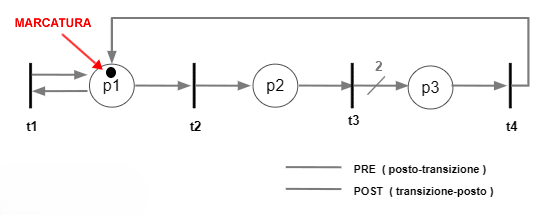
\includegraphics{imgGrafi/marcatura-rete-petri-esempio.png}
\end{center}


\section{Grafi nel machine learning}

Il machine learning sui grafi coinvolge una serie di compiti fondamentali, tra cui la classificazione dei nodi, la previsione degli archi e il clustering. Questi compiti permettono di sfruttare le caratteristiche strutturali dei grafi per fare previsioni, scoprire relazioni nascoste e organizzare i dati in modo significativo. La classificazione dei nodi, ad esempio, mira a prevedere le etichette dei nodi basandosi sulle loro caratteristiche e connessioni. Questo tipo di analisi trova applicazioni comuni nell'identificazione di utenti fraudolenti nei social network o nella classificazione delle proteine nelle reti biologiche.

\subsection{Classificazione dei nodi}

La classificazione dei nodi è uno dei compiti principali nel machine learning sui grafi. In questo contesto, l'obiettivo è prevedere l'etichetta di un nodo sconosciuto basandosi su un piccolo insieme di nodi etichettati e sulle caratteristiche strutturali del grafo. Questa tecnica è ampiamente utilizzata nei social network, dove è possibile classificare gli utenti in base alle loro connessioni e attività. Ad esempio, l'analisi delle reti sociali può identificare potenziali account fraudolenti attraverso pattern di connessione sospetti o raccomandare contenuti personalizzati agli utenti basandosi sulle loro interazioni. Nei contesti biologici, la classificazione dei nodi può essere utilizzata per identificare tipi di cellule o classi di proteine, migliorando la comprensione delle reti biologiche complesse.

\subsection{Previsione degli archi}

La previsione degli archi è un altro compito cruciale nel machine learning sui grafi. Essa consiste nel prevedere la probabilità che un arco esista tra due nodi non collegati. Questa capacità è particolarmente utile nei sistemi di raccomandazione, dove si possono suggerire nuove connessioni tra utenti o prodotti basandosi su interazioni passate e caratteristiche comuni. Nei contesti biologici, la previsione degli archi può facilitare la scoperta di nuove interazioni tra proteine o la previsione di reazioni chimiche, accelerando la ricerca scientifica e lo sviluppo di nuovi farmaci. Inoltre, questa tecnica è applicabile in molte altre aree, come la previsione di collaborazioni in reti di ricerca o l'identificazione di link mancanti in reti di trasporto.

\subsection{Reti neurali sui grafi}

Le reti neurali sui grafi (GNN) sono una classe avanzata di reti neurali progettate per effettuare inferenze su dati strutturati come grafi. Le GNN generalizzano il concetto di reti neurali convolutive ai grafi, permettendo l'estrazione di caratteristiche dai dati strutturati a grafo in modo efficace. Esse utilizzano un processo di aggregazione dei vicini per aggiornare le rappresentazioni dei nodi, catturando così le dipendenze locali e globali nei grafi. Questa capacità di modellare relazioni complesse rende le GNN particolarmente potenti in molte applicazioni.

Le GNN hanno trovato applicazioni in una vasta gamma di settori, tra cui la sintesi chimica, dove aiutano a prevedere la formazione di nuove molecole, e la visione 3D, dove migliorano la comprensione delle strutture tridimensionali. Nei sistemi di raccomandazione, le GNN possono suggerire prodotti o contenuti basandosi su pattern di interazione complessi. Inoltre, vengono utilizzate nel question answering, dove aiutano a trovare risposte accurate a domande basandosi su grafi di conoscenza, e nell'analisi delle reti sociali, dove forniscono approfondimenti sulle dinamiche delle interazioni tra utenti. Grazie alla loro capacità di generalizzare su vari domini, le GNN rappresentano una delle tecniche più promettenti per il deep learning su dati a grafo.

\subsection{Metodi di aggregazione e passaggio di messaggi}

Le GNN utilizzano vari metodi di aggregazione per combinare le informazioni dai nodi vicini. Tra i metodi più comuni vi sono l'aggregazione media, dove le informazioni dai vicini vengono mediate per ottenere una rappresentazione centralizzata, l'aggregazione massima, che seleziona il valore massimo tra i vicini per evidenziare le caratteristiche più prominenti, e l'aggregazione sommatoria, che somma le informazioni dei vicini per catturare l'intero contesto locale.

Il passaggio di messaggi è un'altra componente chiave delle GNN. In questo processo, i nodi scambiano informazioni con i loro vicini per aggiornare le proprie rappresentazioni. Questo scambio iterativo di informazioni permette alle GNN di catturare le dipendenze strutturali nei grafi, migliorando le prestazioni su vari compiti di apprendimento. Il passaggio di messaggi consente di costruire rappresentazioni nodali che riflettono sia le caratteristiche dei nodi stessi che le loro relazioni con i vicini, rendendo le GNN estremamente efficaci nell'analisi dei dati strutturati a grafo.


\end{document}
